\section{Overview}

Historically, the study of atmospheric-pressure plasmas (\acs{app}'s) is
indistinguishable from the study of plasmas as a whole. However, the detail of
the measurements and calculations associated with \acs{app}'s has been limited
by their complexity. From a computational perspective, the high pressure and
number of potential reactions present a difficult challenge. Likewise, the high
pressure can significantly complicate the data analysis for a number of plasma
diagnostics. Aside from the high pressures, the large electric fields, short
time scales, and general randomness of \acs{app}'s make even the most basic
observations a feat.

In the last several decades, some of this has begun to change. High-powered
computing has allowed simulations with remarkable detail. Similarly, advances in
technology has enabled plasma diagnostics in regimes that were experimentally
inaccessible. As a result, the body of knowledge regarding \acs{app}'s has
greatly increased. Sometimes, the motivation for this work is scientific
curiosity. More often, the study of \acs{app}'s has been driven by a broad range
of applications.

Among the first plasma applications were provided by \acs{app}'s: ozone
generation and lighting. Aside from these items, plasma welding, polymer
treatment, combustion, and plasma televisions have become widely accepted.
Meanwhile, a large number of new applications may soon be added to this list,
including: treatment of tissue wounds, altering airflow over airfoils, and
destruction of industrial pollutants.

Unsurprisingly, each case demands a different kind of plasma. The original arc
discharges were created between two graphite rods connected to immense battery
banks. In contrast, a modern research reactor studying plasma-assisted
combustion might use a fast-switching semiconductor circuit. Over the years,
several types of \acs{app}s have been developed for a variety of situations:
dielectric-barrier, corona, thermal arc, RF, microwave, pulsed, and more.

Within this group\footnote{The interested reader is referred to Starikovskaia's
review \cite{Starikovskaia2006} which provides a general overview of \acs{app}'s
in the context of plasma-assisted combustion}, the repetitively-pulsed
nanosecond discharge (\acs{rpnd}) has created considerable interest. Generally
speaking, a \acs{rpnd} is a plasma generated by a repetitive electrical pulse
applied between two electrodes. The pulse voltage is often in excess of one
kilovolt, lasts anywhere from $<1-100$ ns, and is repeated over a thousand
times each second. The result is a wave of ionization (and light) which crosses
from the powered electrode to the grounded one.

A \acs{rpnd} can fill volumes of several liters with a relatively uniform
plasma. Though they can cause significant excitation of the background gas, they
generally produce very little heating (in some cases below a detection limit of
$\Delta \pm 15$ K). In addition, the excitation can be changed with adjustments
to the magnitude or duration of the electrical pulse. Each of these
characteristics are highly desirable in one or more of potential applications
for \acs{app}'s.

Given all of these promising properties, \acs{rpnd}'s have been the subject of
substantial study by several research groups. However, much of this work has
focused on the physics of \acs{rpnd}'s in air. Unfortunately, air's large number
of constituent elements can lead to notable complexity. In turn, this can
obscure some of the more fundamental questions relation to \acs{rpnd}'s: how do
they form, how is the energy distributed between excited particles, and what
kind of spatial variation can be expected?

This paper details a study of each of these questions in a helium \acs{rpnd}.
Specifically, the densities of one particular excited atom are measured for a
variety of pressures and locations. This is complemented by measurements of the
light emissions for the same set of parameters. A simple model of a \acs{rpnd}
is used to predict several characteristics of the plasma based on the excited
state densities: electron density, electric field, and light emission. The
measured light emissions are interpreted to show how the energy is distributed
in the gas, and how it changes over time. Finally, they are compared with the
estimated light emissions to check the validity of several common assumptions.

\section{Literature Review}

\acs{rpnd}'s are only a recent invention which resulted from advances in
fast-switching semiconductors. However, the physics of their formation is
related to a much larger category of plasmas which includes lightning, sparks,
and even some transient phenomena in DC glows. These plasmas are unique in that
their formation occurs on timescales much faster than the traditional Townsend
mechanism allows for. The means by which these plasmas form has acquired several
names in the literature; here we will adopt the term, fast ionization wave
(\acs{fiw}).\footnote{It should be noted that the phrase wave does not indicate
any kind of periodic motion or spatial arrangement. Simply put, it describes a
boundary which separates ionized and unionized gas which travels from one
electrode to another.}.

\subsection{Early History of Pulsed Discharges}

The first \acs{fiw} was likely generated by Wheatstone in 1835
\cite{Wheatstone1835}. As reported by Thomson \cite{Thomson1893}, Wheatstone
built a vacuum tube six feet in length, and applied a high voltage across the
gas. As a plasma formed in the tube, Wheatstone observed its formation with a
rotating mirror. The use of this apparatus allowed Wheatstone to place a lower
limit on the speed with which the plasma travelled from one electrode to the
other. Though the discharge crossed the tube with a speed of at least
$8\times10^7$ cm/s, spectral observations indicated that the particles emitting
the light were not travelling at that speed \cite{Zahn1879}.

Later, Thomson revisited this work with an improved apparatus
\cite{Thomson1893}. This included a tube that was now 15 m in length and five mm
in diameter, as seen in figure \ref{fig:thomson}.
\begin{figure}
  \centering
  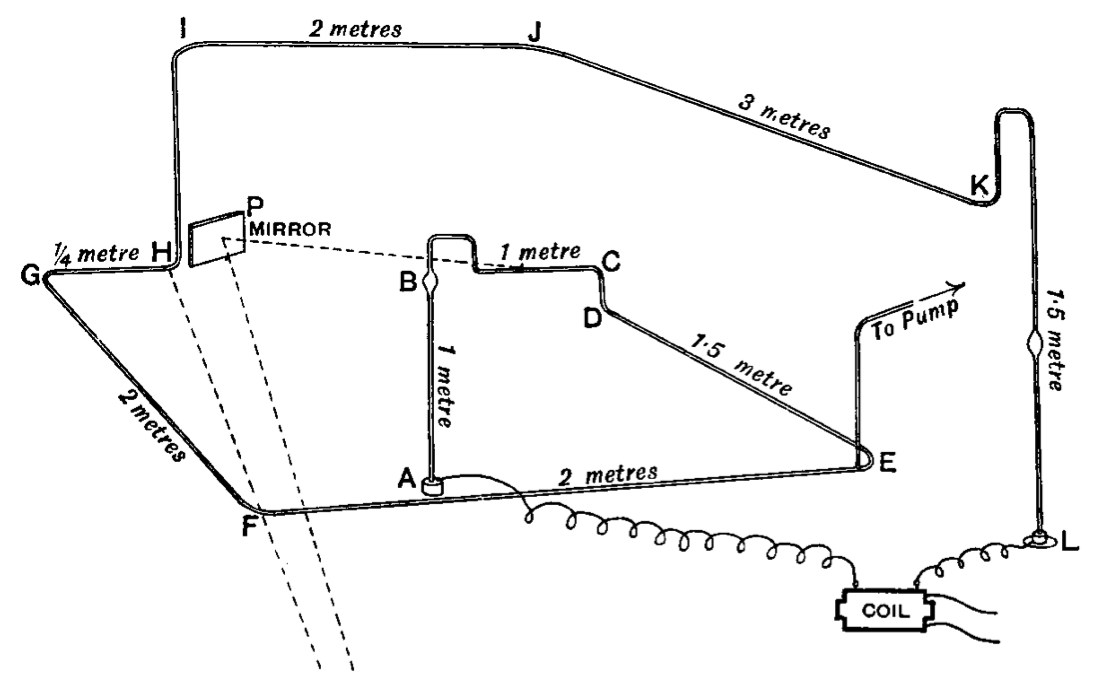
\includegraphics[width=4in]{chapters/introduction/figures/thomson.png}
  \caption{A sketch of J.J. Thomson's early experiments on fast ionization
  waves in long vacuum tubes.}\label{fig:thomson}
\end{figure}
Also using the rotating mirror apparatus, Thomson was able to greatly improve on
the estimates of Wheatstone. He estimated that the so-called ``luminous front''
had a speed that was more than $1.5\times10^{10}$, or in excess of half of the
speed of light. Furthermore, Thomson determined that the front always appeared
to travel from the positively pulsed electrode (anode) to the ground electrode
(cathode).

The study of these luminous fronts was revisited by several researchers in the
wake of Thomson \cite{James1904, Whiddington1925, Beams1926} with varied
success. By his own admission, Beams's work in 1926 was done ``hurriedly,''
using a rudimentary Kerr cell. In 1930, Beams returned to the propagation of
light pulses in vacuum tubes with a rotating mirror apparatus \cite{Beams1930}.
In addition to confirming his previous measurements, and those of Thomson, Beams
discovered that the \acs{fiw} always traveled from the electrode with the
highest absolute potential, to the lowest one. In other words, the wave could be
anode or cathode directed, depending on the magnitude of their potentials
relative to ground. Benefiting from an improved understanding of electricity,
namely the existence of electrons and ions, Beams was able to provide the first
hypothesis on the nature of the \acs{fiw}:
\begin{quote}
  In the neighborhood of the electrode $\ldots{}$ the field is very high and
  intense ionization should take place. This ionization due to the large
  difference in mobilities of positive ions, negative ions and electrons
  respectively should result in the establishment of a space charge. This space
  charge, once formed near the high potential electrode $Q$ must move down the
  tube regardless of the polarity of the applied potential because of the
  changes it produces in the field near its edges.
\end{quote}

At about the same time, Schonland and Collens reported on their observations of
lightning \cite{Schonland1933}. Though the general structure and length scale of
lightning is substantially different from the luminous fronts observed by Beams
and Thomson, the two phenomena would later prove to be very similar. In their
work Schonland and Collens noted that lightning would usually occur in a
two-step process. Based on the images they obtained, they suggested that
the leader was generated by a relatively small ``dart'' with a mean vertical
velocity of $7.2\times10^8$ cm/s. The dart moved in a random manner, changing
directions at random intervals, but always moving downward.

The second step began when this dart reached the ground. Once there, a bright
return stroke would occur along the same path that the leader had traced out. In
contrast to the leader stroke, the return stroke had a velocity of $5\times10^9$
cm/s. Schonland and Collens hesitantly attributed the leader stroke to an
extended electron avalanche, and the return stroke to thermal ionization along
the conductive path generated by the dart. However, calculations by Cravath and
Loeb showed that the speeds of the proposed avalanche would have to be
inconsistent with the fields at the head of a lightning stroke
\cite{Cravath1935}. Instead, they suggested that the dart was actually a moving
region of space charge which locally accelerated electrons to ionizing energies.
This was fundamentally similar to the mechanism proposed by Beams in 1930.

\subsection{The Streamer Model}

It was long known that sparks in air were similar to lightning. Advances in
technology during the 1930's led to experiments which reinforced this
similarity. In response to the measurements of Schonland and Collens; Snoddy,
Beams, and Dietrich studied the breakdown of gas in a long tube with an
oscillograph \cite{Snoddy1936}. The results from the oscillograph showed a very
clear return wave for which they measured several parameters the characterized
as a function of pressure and applied potential. They observed that at low
voltages, the system behaved like a large resistor in series with a capacitor,
and below a critical voltage, no return stroke would form. Finally, in order to
explain the propagation of the \acs{fiw} generated by the positive pulse, they
suggested that photoionization was occurring in the space ahead of the wave.

Around the same time, Flegler and Raether had come to a similar conclusion,
leading to the first attempt at a theory describing streamers
\cite{Flegler1936}. This same theory was proposed independently by Loeb and Meek
in a series of papers \cite{Loeb1940, Loeb1940a, Meek1940}. The streamer theory
divided the initial breakdown of a spark into two steps. In the first step, an
electron avalanche is initiated between two electrodes. The avalanche travels
toward the anode and leaves behind a region of high positive space charge. In
the second step, the return stroke begins at the cathode and travels toward the
cathode. It was suggested that the head of the return stroke ionizes the gas
ahead of it by pulling in background electrons or via photoionization.
\footnote{These early works emphasized the importance of photoionization. It is
now know that it is only required for cathode-directed streamers in systems with
no background ionization. In addition, Mesyats later showed that the lifetime of
the excited states responsible for photoionization were often longer than the
lifetime of the streamers \cite{Mesyats1972}}.

The streamer model proved relatively successful in describing the development of
sparks and lightning. Theoretical estimates of the speed matched the velocity
measurements that were acquired through photographs and oscillographs.
Additionally, the theory is able to account for the halting manner in which
lightning is formed, though it is only tentatively able to describe the
branching and stepped appearance. Finally, the streamer mechanism provides an
adequate explanation of why streamer discharges are not affected by the shape or
material of the cathode, namely, they do not depend on secondary electron
emission.

The study of the formation of streamers and lightning continues to be active to
this day. Following the initial work of Flegler, Raether, Loeb, and Meek, a
number of researchers began to explore the boundary between the Townsend
mechanism and the streamer mechanism, e.g. Fisher and Bederson's work in 1951
\cite{Fisher1951}. However, there were still a number of phenomena that were
poorly explained by the streamer model. In particular, Kunhardt provided a
useful overview of the problems in 1980 \cite{Kunhardt1980}. However, even
before that, it was apparent that the transients of sparks and lightning was
more complicated than thought.

\subsection{Transient Glow Discharges}

Per Chalmers \cite{Chalmers1971}, Rogowski and Buss \cite{Rogowski1927,
Buss1932} observed a diffuse glow discharge immediately prior to the filaments
which often accompany a streamer discharge. Likewise, Allibone and Meek, noted
extremely diffuse discharges in air as seen in oscillographs and photographs
\cite{Allibone1938, Allibone1938b, Allibone1938c}. However, the Boys apparatus
which was used to obtain photographs of the streamer was unable to capture the
evolution of the diffuse glow, given its large spatial extent.

This was first noted by Allibone who attempted to use Lichtenberg figures to
demonstrate this diffuse glow \cite{Allibone1948}. Later, Saxe and Meek used the
recently invented photomultiplier tube to record the evolution of the light
emissions in the transient diffuse glow \cite{Saxe1948} as a function of space.
Both studies concluded that there was a diffuse glow which crossed the gap which
immediately precluded the formation of the leader streamer.



As an aside, the topic of electron beams in rare gases became of substantial
interest to researchers in the mid 1970s. Because rare gases lacked low-lying
excited states which might detrimentally absorb energy, they were favor for
laser where a population inversion could be achieved with ease. As a result, a
great deal of work went into detailing the propagation of an electron beam in
rare gases which is physically similar to the development of a fast ionization
wave. However the primary difference between

It was around this time that the topic of fiw became of substantial interest to
Russian research groups. Though much of the early work is shrouded in the mists
of language differences, it is believed that Vasilyak \cite{Vasilyak1994}
provides a fair review of the material. 

Come 1998, the fiw was the subject of renewed interest by a group of researchers
at the Moscow Institute of Physics and Technology \cite{Anikin1998}. They
employed several different diagnostic techniques (photomultiplier tubes and
capacitive probes) in an exceptionally detailed study of fiws in both air and
nitrogen, using a shock tube and a bell jar. A summary of these investigations
can be found in \cite{Starikovskaia2001}. The work showed exceptionally
reproducibility of the discharge parameters at relatively low repetition rates,
on the order of tens of Hz, and evidence of runaway electrons in the
electronically excited molecular states. This work also included some of the
first approximations of the electron energy distribution function (\acs{eedf}).
This was found by comparing several paremeterized distribution functions with
the resulting excited state populations. 

This was time the population kinetics of an fiw was really examined. In this
case, it emphasized the short-lived states of nitrogen. Specifically,
\cite{Pancheshnyi1998} initially used the fiw to examine the population of
electronic states of nitrogen. Later analysis \cite{Pancheshnyi1999} concluded
that the, for a negative fiw in nitrogen, the vast majority of the electrons
were generated in the aftermath of the wave and that the ionization did not
track the luminous front. Additionally, measurements of the conductivity
suggested that the local approximation becomes invalid in the wave front and the
electron energy distribution function resembles a beam.

The insufficiency of photionization was later reinforced by the observation of
Mesyats \cite{Mesyats1972} that the speed of the discharge processes was often
faster than the lifetimes of excited states. Again, this precluded
photoionization from providing a significant amount of preionization for the
propagation of an rpnd. Mesyats instead suggested that the large fields
generated an electron avalanche that grew much more rapidly than the typical
Townsend discharge. This was followed by an avalanche chain which further
propagated the plasma.

This explanation 

Later, Kunhardt \cite{Kunhardt1980} extended on Mesyats' analysis and provided a
more theoretical underpinning for it. Taking his inspiration from the group
theory used in neutron diffusion, Kunhardt explored the development of a fiw
from the perspective of ``trapped'' and ``runaway'' electrons. In his
work, Kunhardt identifies th

Previous work by
Babich and Stankevich \cite{Babich1973} inspired this by suggesting the
existence of continually-accelerated electrons at high overvoltages.


\subsection{rpnds}

The development of fid semiconductor technology in the late 1990's and their
commercialization in the early 2000's allowed the use of rpnds. Fundamentally,
these discharges were the same as the fiws that had been studied for decades
earlier. However, the much greater repetition rates (on the order of tens of
kHz), meant that the discharges could be used in a number of previously
impossible applications. Attention quickly turned toward plasma-assisted
combustion \cite{Starikovskaia2006}, mhd energy bypass \cite{Macheret2002}, and
later, plasma actuators \cite{Adamovich2009}. Additionaly studies, related to
the development of high-pressure xenon lamps, led to several more quantitative
models of the fiw development \cite{Nikandrov2008, Tsendin2009}. These works
also contributed to a semi-analytical energy coupling model as well
\cite{Adamovich2009}.

Research efforts continued to use many of the same diagnostics as before. The
current and voltage at the powered electrode were recorded (with varying levels
of diligence), electric fields were measured with capacitive probes, and
photomoultiplier tubes were used to measure the progress of the luminous front.
The 2000's did add a few new tools to the diagnostic arsenal. Perhaps the most
common addition is the use of ICCD's in order to record transition and broadband
light. This approach has been used to verify the reproducibility of the
discharge \cite{Adamovich2009}. Though the gate times are still too short to
capture the development of the wave, excitation profiles like those initially
demonstrated by Vasilyak\cite{Vasilyak1994} are commonly recorded. Another, more
exotic addition, has been the use of CARS. This nonlinear technique has proven
to be excellent at reproducing the spatial temperature profiles of pulsed
nanosecond discharges. This has become particularly interesting for groups
interested in applications to fast gas heating \cite{Zuzeek2010}. Others have
used CARS to explore the electric field development of rpnds \cite{Ito2010,
Ito2010a}. Finally, another research group has used LCIF to detect the radial
and axial profiles of the metastable and electron densities in a helium
discharge. The CARS and LCIF approaches are both notable for being active
diagnostics of direct properties. This allows unprecedented time resolution and
detail.



